115. \begin{figure}[ht!]
\center{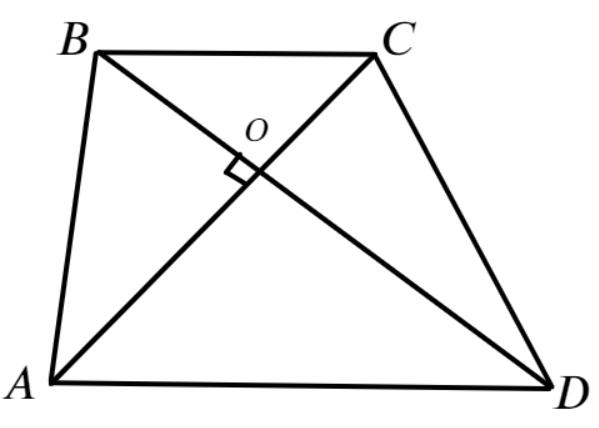
\includegraphics[scale=0.35]{g8-115.png}}
\end{figure}\\
Треугольники $AOB,\ BOC,\ COD$ и $AOD$ являются прямоугольными. Пусть $AO=x,\ CO=4-x,\ BO=y,\ DO=5-y.$ Тогда $S_{ABCD}=S_{\Delta AOB}+S_{\Delta BOC}+S_{\Delta COD}+S_{\Delta AOD}=\cfrac{xy}{2}+\cfrac{y(4-x)}{2}+\cfrac{(4-x)(5-y)}{2}+\cfrac{x(5-y)}{2}=\cfrac{xy+4y-xy+20-4y-5x+xy+5x-xy}{2}=10.$\\
